\chapter{Study 2: A Selective Backward Pass}\label{ch:study2}

This chapter answers RQ3. It starts from the measurement of \cref{sec:concentration}, reports the exploratory looks that shaped the pre-registered design, and then reports the confirmatory test.

\section{From a measurement to a hypothesis}\label{sec:s2-lead}
\paragraph{Pilot.} The concentration of the gradient on a few high-loss rows suggested a simple arm: run the forward pass on all rows, back-propagate only the highest-loss $30\%$ (S30) or $50\%$ (S50), and compare with a random subset of the same size (R30). A pilot on three new seeds (\tierE{}; the decision rule was fixed before the run) gave mean FLOPs-to-target of $0.634$, $0.768$ and $1.413$ times that of the tuned baseline at $0.97$ for S30, S50 and R30, and $0.612$, $0.707$ and $1.181$ at $0.975$. Selecting rows by loss is what kept the number of steps low: the random control was worse than the baseline.

\paragraph{Three exploratory looks.} Three further looks (\tierE{}, three seeds each) tested the points on which the pilot was most open to objection.
\begin{enumerate}
\item \emph{Is it just a batch-size effect?} Selecting $30\%$ of a batch of 128 means back-propagating about 39 rows, so a plain baseline with a smaller batch costs about the same per step. A baseline at batch 48 (with a lighter tuning) needed $0.889$ and $0.921$ of the FLOPs of the batch-128 baseline, and S30 $0.778$ and $0.652$; against the best small batch, S30's advantage fell to $0.876$ at $0.97$ and $0.708$ at $0.975$. This made a fully tuned small-batch arm a necessary reference.
\item \emph{How many rows to keep?} FLOPs-to-$0.975$ was flat for kept fractions between $0.1$ and $0.3$ (ratios of $0.58$ to $0.63$ of the baseline) and worse at $0.5$ (\cref{fig:s2-controls}a). Keeping fewer rows lowers the cost per step but raises the number of steps, and the product stays roughly constant.
\item \emph{Does the saving translate into time?} See \cref{sec:wallclock}.
\end{enumerate}

\begin{figure}[t]
\centering
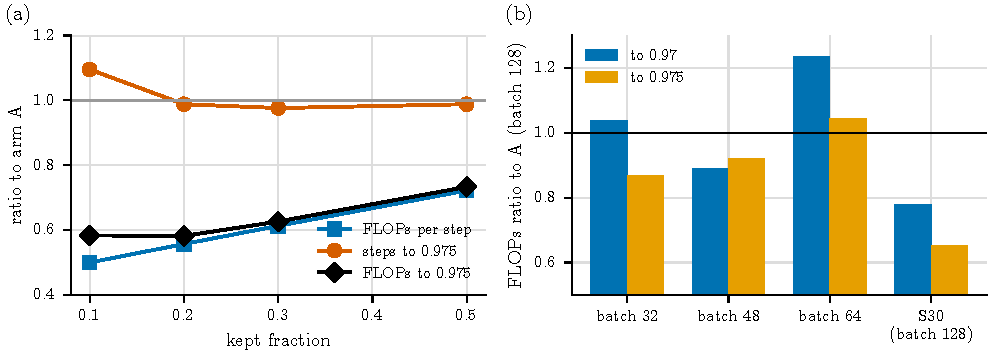
\includegraphics[width=\textwidth]{fig_s2_controls}
\caption{Exploratory looks that shaped the Study~2 design (3 seeds each; $\mathcal{E}$ tier). (a) Kept fraction: the exact cost per step falls with the fraction, the number of steps to $0.975$ rises, and their product, the FLOPs-to-target, is flat between $0.1$ and $0.3$. (b) A plain smaller batch (b32, b48, b64; lightly tuned) against the batch-128 baseline and S30: a smaller batch is not clearly better than batch 128, but it narrows S30's advantage.}
\label{fig:s2-controls}
\end{figure}

\section{The pre-registered design}\label{sec:s2-design}
The second pre-registration (tag \code{prereg-v2}, \cref{tab:prereg}) fixed two confirmatory hypotheses:
\begin{description}[leftmargin=2.6em,style=nextline]
\item[H7a] S30, with the hyper-parameters of the baseline A1, needs at least $15\%$ fewer FLOPs-to-target than A1 at both $0.97$ and $0.975$.
\item[H7b] S30 needs fewer FLOPs than the \emph{fully tuned best small-batch baseline} (margin $0\%$): a control for ``is the gain only a batch-size effect''.
\end{description}
S30 keeps $30\%$ of the rows, uses a warm-up of 100 full steps, and \emph{inherits A1's hyper-parameters}; this is conservative because A1 was tuned and S was not. 20 paired seeds (1300--1319) were used in 11 groups (220 runs).

\subsection{Six tunings of the baseline}\label{sec:retune}
Because Study~1 showed that a single tuning can mislead (\cref{sec:noise}), the baseline was tuned six times with independent seeds and trials (A1, A2, A5--A8), all six were re-run on the Study~2 seeds, and the batch-48 arm B48 was tuned with the same 25-trial search space (batch 48, 8\,000 steps so that it sees the same number of samples as 3\,000 steps at batch 128, evaluated every 125 steps).

\section{Results}\label{sec:s2-results}
\begin{table}[t]
\centering\small
\caption{Study 2: mean GFLOPs-to-target, mean steps among the runs that reached the target, runs that never reached it, and paired change against A1 ($97.5\%$ bootstrap intervals), 20 seeds per group. Steps of B48 are steps at batch 48 (8\,000-step horizon) and are not comparable with the others. S20, S30T and R30 are descriptive.}
\label{tab:s2-main}
\resizebox{\textwidth}{!}{%
\begin{tabular}{@{}l rrr l rrr l@{}}
\toprule
 & \multicolumn{4}{c}{target 0.97} & \multicolumn{4}{c}{target 0.975}\\
\cmidrule(lr){2-5}\cmidrule(l){6-9}
Group & GFLOPs & steps & never & change (\%) & GFLOPs & steps & never & change (\%)\\
\midrule
A1 (tuned baseline) & 147.7 & 952 & 0 & -- & 219.4 & 1415 & 0 & -- \\
A2 & 186.5 & 1202 & 0 & $+26.2$ [$+18.5$, $+34.7$] & 248.9 & 1605 & 0 & $+13.4$ [$+4.9$, $+22.5$] \\
A5 & 139.6 & 900 & 0 & $-5.5$ [$-12.5$, $+0.0$] & 212.8 & 1372 & 0 & $-3.0$ [$-8.3$, $+2.0$] \\
A6 & 146.1 & 942 & 0 & $-1.0$ [$-7.8$, $+6.3$] & 212.0 & 1368 & 0 & $-3.4$ [$-11.3$, $+4.6$] \\
A7 & 143.8 & 928 & 0 & $-2.6$ [$-10.6$, $+5.5$] & 210.9 & 1360 & 0 & $-3.9$ [$-8.9$, $+0.8$] \\
A8 & 157.0 & 1012 & 0 & $+6.3$ [$-1.0$, $+14.5$] & 227.2 & 1465 & 0 & $+3.5$ [$-2.6$, $+10.3$] \\
\midrule
B48 (tuned batch 48) & 137.4 & 2362 & 0 & $-7.0$ [$-13.7$, $+0.2$] & 209.3 & 3600 & 0 & $-4.6$ [$-11.9$, $+3.6$] \\
\midrule
S30 (selective, kept 0.3) & 95.9 & 945 & 0 & $-35.1$ [$-38.6$, $-31.5$] & 135.1 & 1358 & 0 & $-38.4$ [$-41.2$, $-35.6$] \\
\midrule
S20 (kept 0.2, descriptive) & 88.2 & 942 & 0 & $-40.3$ [$-43.0$, $-37.7$] & 125.4 & 1372 & 0 & $-42.9$ [$-46.2$, $-39.2$] \\
S30T (S tuned once, descriptive) & 92.5 & 910 & 0 & $-37.4$ [$-40.6$, $-34.2$] & 139.8 & 1408 & 0 & $-36.3$ [$-39.9$, $-32.2$] \\
R30 (random 30\%, control) & 186.4 & 1898 & 0 & $+26.2$ [$+19.0$, $+34.3$] & 251.1 & 2503 & 3 & $+14.4$ [$+8.3$, $+21.4$]
\\
\bottomrule
\end{tabular}}
\end{table}

\begin{keyfinding}
\textbf{H7a and H7b are supported.} Back-propagating only through the $30\%$ highest-loss rows needed $35.1\%$ ($[-38.6,-31.5]$) fewer FLOPs than the tuned baseline to reach $0.97$ and $38.4\%$ ($[-41.2,-35.6]$) fewer to reach $0.975$, and $30.2\%$ ($[-35.7,-24.3]$) and $35.5\%$ ($[-39.8,-30.9]$) fewer than the fully tuned batch-48 baseline. It was cheaper than A1 in 20 of 20 seeds at both targets, and cheaper than B48 in 20 of 20.
\end{keyfinding}

\paragraph{The shift rule is not binding.} The largest reduction achieved by any of the five re-tunings against A1 was $5.5\%$ at $0.97$ and $3.9\%$ at $0.975$ (\cref{tab:s2-main}); both are far smaller than S30's gain of $35$--$38\%$. The second tuning A2 is $+26.2\%$ and $+13.4\%$ \emph{worse} than A1 on these seeds, which reproduces the Study~1 finding that tunings of the same baseline differ much more than seeds do.

\paragraph{Controls.} The random control R30 keeps $30\%$ of the rows at random and needs $26.2\%$ and $14.4\%$ \emph{more} FLOPs than A1, and fails to reach $0.975$ in 3 of 20 seeds, so the selection by loss is what makes the pass work: back-propagating the same number of rows chosen at random is worse than the full pass. The tuned small batch B48 is $-7.0\%$ ($[-13.7,+0.2]$) and $-4.6\%$ ($[-11.9,+3.6]$) against A1, which is not a clear gain, as in the exploratory look. \Cref{fig:s2-curves}a shows that S30 reaches every accuracy level earlier in FLOPs, and \cref{fig:s2-curves}b that the per-seed ratio is below $0.85$ for every seed.

\begin{figure}[t]
\centering
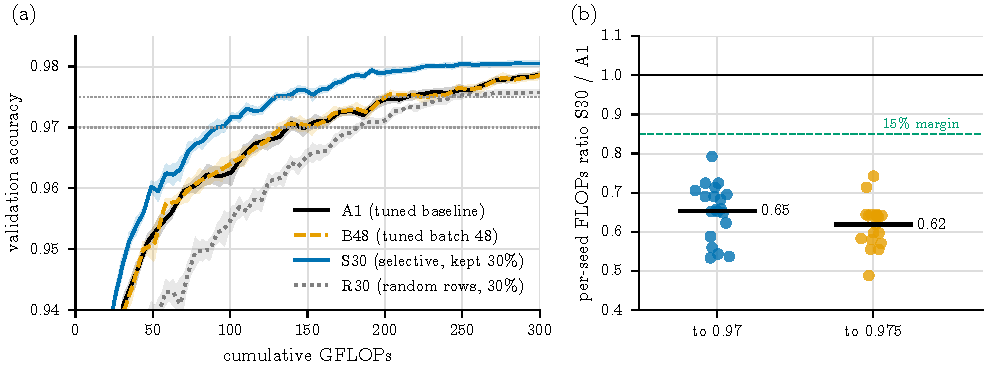
\includegraphics[width=\textwidth]{fig_s2_curves}
\caption{Study 2. (a) Validation accuracy against cumulative GFLOPs for the baseline A1, the tuned batch-48 baseline, S30 and the random control, mean of 20 seeds with $95\%$ bands. (b) Per-seed FLOPs ratio S30/A1 at the two targets (black bar: mean of the per-seed ratios); the dashed line is the pre-registered $15\%$ margin.}
\label{fig:s2-curves}
\end{figure}

\paragraph{Where the saving comes from.} S30 needs about the same number of steps as A1 ($945$ and $1358$ against $952$ and $1415$). Its saving is therefore almost entirely the lower cost per step ($0.613$ of A1's), and the pre-registered question was whether the number of steps stays near the baseline's across seeds and tunings. It does.

\section{Exploratory contrasts on the same seeds}
Two descriptive groups were run on the same seeds. Keeping $20\%$ of the rows (S20) saved a further $7$--$8\%$ over S30 at the same number of steps ($-7.9\%$ at $0.97$, $-7.2\%$ at $0.975$ against S30; a post-hoc contrast, so a lead and not a claim). S30 with its own tuning (S30T, tuned once over the baseline's search space) was no better than S30 with the baseline's settings ($-37.4\%$ and $-36.3\%$ against A1), so the inherited configuration is not an obstacle. The warm-up of 100 full steps accounts for about $11$--$12\%$ of the FLOPs to $0.975$ and had never been varied; this led to Study~3.

\section{Does a FLOPs saving translate into time?}\label{sec:wallclock}
FLOPs do not count the top-$k$ selection, the gather of rows, or the interpreter overhead of a small model. Time per step was therefore measured separately (\tierE{}: one seed, one CPU, 200 warm-up and 1\,000 timed steps, 3 repeats, alternating the arms; the rule was fixed before the run). The median time per step of S30 over A was $0.825$ with one torch thread and $0.914$ with eight, against an exact FLOPs ratio of $0.613$ (\cref{fig:metrics}b). The saving in time per step is therefore about $45\%$ (one thread) and $22\%$ (eight threads) of the saving in FLOPs. The one-thread value is within the noise of the rule's threshold (per-repeat ratios $0.61$, $0.92$, $0.81$, the first A repeat being a cold start). A rough, \emph{derived and not measured} estimate of the time to target multiplies the per-step ratio by the step ratio ($0.98$ to $1.20$ in the exploratory looks): about $0.8$ to $1.0$ of the baseline's time at one thread and $0.9$ to $1.1$ at eight, so the wall-clock gain \emph{could vanish} at this model size. The time column of the run logs includes evaluation passes and cannot be used for this. A larger model, a GPU, or an implementation that fuses selection with the forward pass may differ; none was measured. The report therefore claims a saving in counted FLOPs, not in time.

\section{Summary of Study 2}
In a pre-registered test with six tunings of the baseline, a fully tuned small-batch baseline and a random-rows control, back-propagating only through the highest-loss $30\%$ of each batch reduced the FLOPs needed to reach $0.97$ and $0.975$ by $35$--$38\%$ against the baseline and by $30$--$36\%$ against the small-batch baseline, in every one of 20 seeds. The idea is known (\cref{sec:related-selection}); the contribution is the controlled confirmation, with the baseline's tuning noise and the batch-size explanation built in. The measured saving in time per step is much smaller than the saving in FLOPs.
